%% It is just an empty TeX file.
%% Write your code here.
% !TEX encoding = UTF-8 Unicode
\documentclass[a4paper, 12pt]{article}   	% use "amsart" instead of "article" for AMSLaTeX format
\usepackage[left=20mm, top=15mm, right=10mm, bottom=15mm]{geometry}    

            
\usepackage[parfill]{parskip}    		% Activate to begin paragraphs with an empty line rather than an indent
\usepackage{graphicx}				% Use pdf, png, jpg, or eps§ with pdflatex; use eps in DVI mode
\usepackage[14pt]{extsizes}
\usepackage{setspace,amsmath}
\usepackage{ dsfont }
\usepackage{graphicx}
\renewcommand{\labelenumii}{\theenumii}
\renewcommand{\theenumii}{\theenumi.\arabic{enumii}.}
\usepackage{amsmath,amssymb}
\usepackage[unicode]{hyperref}

\usepackage{xcolor}
\usepackage{color}
\usepackage{minted}
\usepackage{caption}

\usepackage{array}
\newcolumntype{P}[1]{>{\centering\arraybackslash}p{#1}}

\usepackage{cmap} % Улучшенный поиск русских слов в полученном pdf-файле
\usepackage[T2A]{fontenc} % Поддержка русских букв
\usepackage[utf8]{inputenc} % Кодировка utf8
\usepackage[english, russian]{babel} % Языки: русский, английский

								% TeX will automatically convert eps --> pdf in pdflatex		
\usepackage{amssymb}

\begin{document}
\begin{titlepage}

\thispagestyle{empty}

\begin{center}
Федеральное государственное бюджетное образовательное учреждение высшего профессионального образования Московский государственный технический университет имени Н.Э. Баумана
\end{center}


\vfill

\centerline{\large{Лабораторная работа №4}}

\centerline{\large{«Оценка полученного дохода Пражского метро»}} 

\centerline{\large{по курсу}}
\centerline{\large{«Моделирование»}}


\vfill

Студент группы ИУ9-82 \hfill Белогуров А.А.

Преподаватель \hfill Домрачева А.Б.
\vfill

\centerline{Москва, 2018}
\clearpage
\end{titlepage}

\newpage
\setcounter{page}{2}

\tableofcontents

\newpage

\section{Цель работы}
    Ознакомиться в математичской моделью, построенной на основе статистических данных и проанализировать полученную модель.
 
\newpage

\section{Постановка задачи}
    Имеются статистические данные пражского метро за 2014 год. Данные представлены в трёх таблицах и отражают информацию о:
    
    \begin{itemize}
        \item $th$ $X$ - кол-во людей, вошедших на станцию $X$ в течение дня, как срендестатистическое за месяц;
        \item $r$ $X$ - кол-во прошедших через турникеты на станции $X$ в течение дня, как срендестатистическое за месяц;
        \item $II$ $X$ кол-во купленных билетов на станции $X$ за месяц;
        \item Общее количество станций - 61.
    \end{itemize}
    
    Билеты распределены по трем категориям:
    \begin{itemize}
        \item $F$ - взрослый билет, стоимость:
        \begin{enumerate}
            \item 30 мин - 24 крон
            \item 90 мин - 32 крон
            \item 24 часа - 110 крон
            \item 72 часа - 310 крон
        \end{enumerate}
        \item $D$ - детский билет, стоимость:
        \begin{enumerate}
            \item 30 мин - 12 крон
            \item 90 мин - 16 крон
            \item 24 часа - 55 крон
            \item 72 часа - 310 крон
        \end{enumerate}
        \item $L$ - льготный билет, стоимость (аналогично десткому).
    \end{itemize}
    
\subsection{Задача 1}
    Проверить, насколько тесна связь между потоком пассажиров вошедших в метро, и пассажиров прошедших через турникеты.
    
    \begin{center}
        \begin{minipage}{0.9\linewidth}
            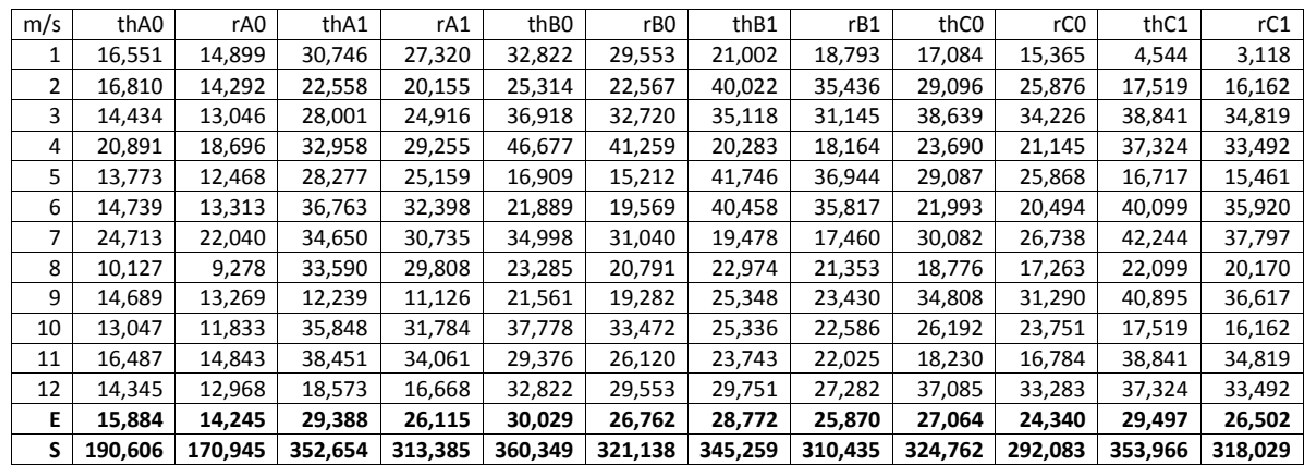
\includegraphics[width=\linewidth]{img/task_1}
            \captionof{figure}{Входные данные задачи 1}
        \end{minipage}
    \end{center}
    
\subsection{Задача 2}
    Оценка общего потока пассажиро на основе данных из русунков 2-5.
    
    Неообходимо:
    \begin{enumerate}
        \item Оценить долю турникетов с памятью среди всех турникетов в метрополитене
        \item Определить связь между количеством человек, вошедших в метро в день контроля, и количеством человек, оплативших проезд.
    \end{enumerate}
    
    \begin{center}
        \begin{minipage}{0.9\linewidth}
            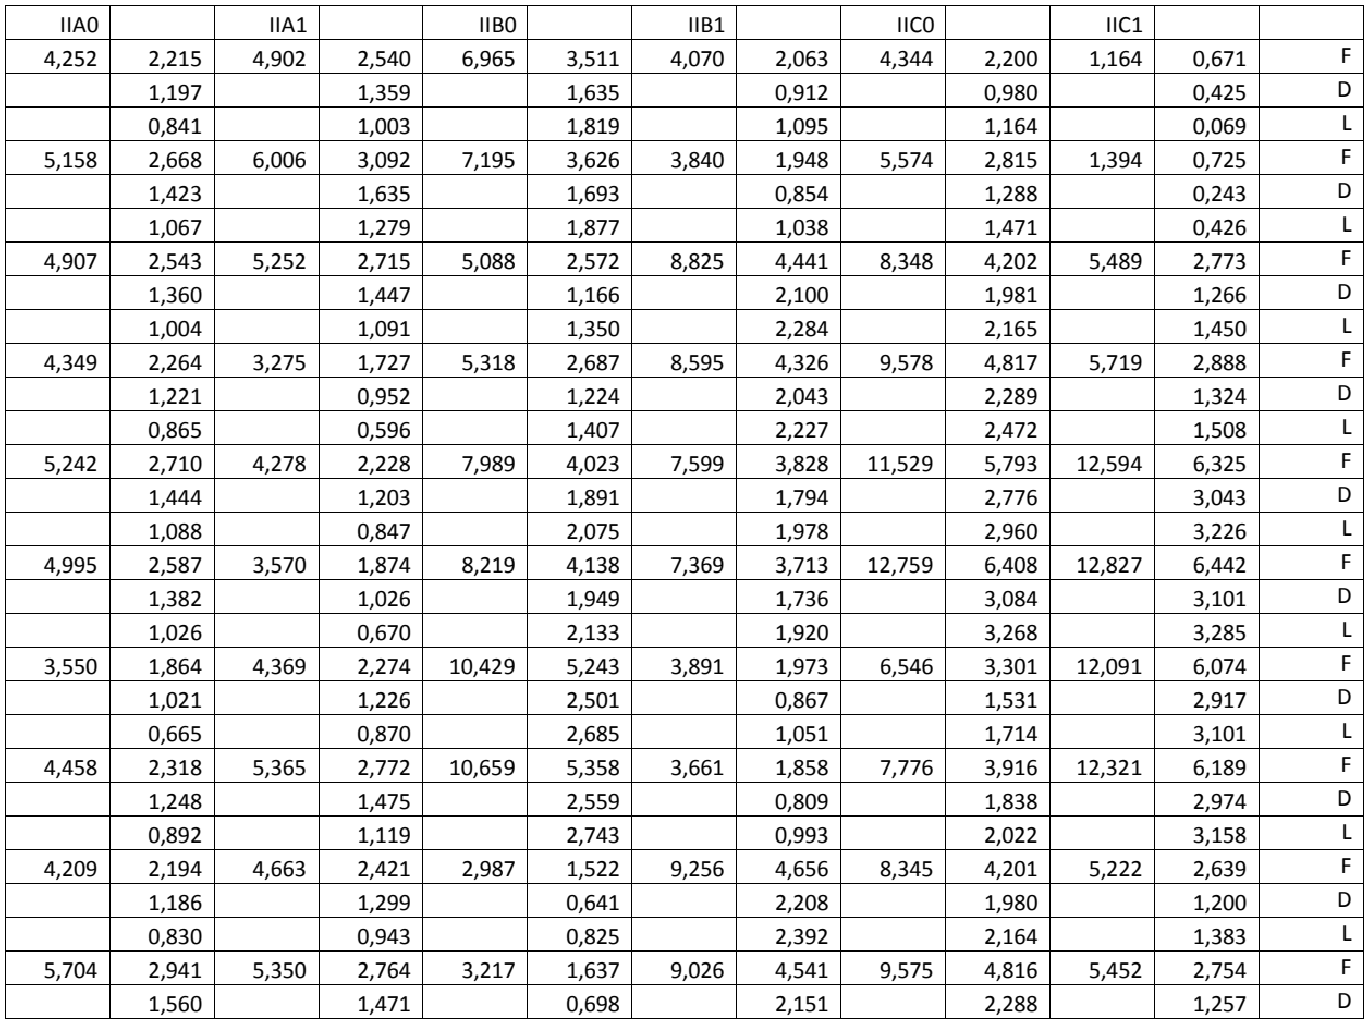
\includegraphics[width=\linewidth]{img/task_2_0}
            \captionof{figure}{Входные данные задачи 2(1)}
        \end{minipage}
    \end{center}
    \begin{center}
        \begin{minipage}{0.9\linewidth}
            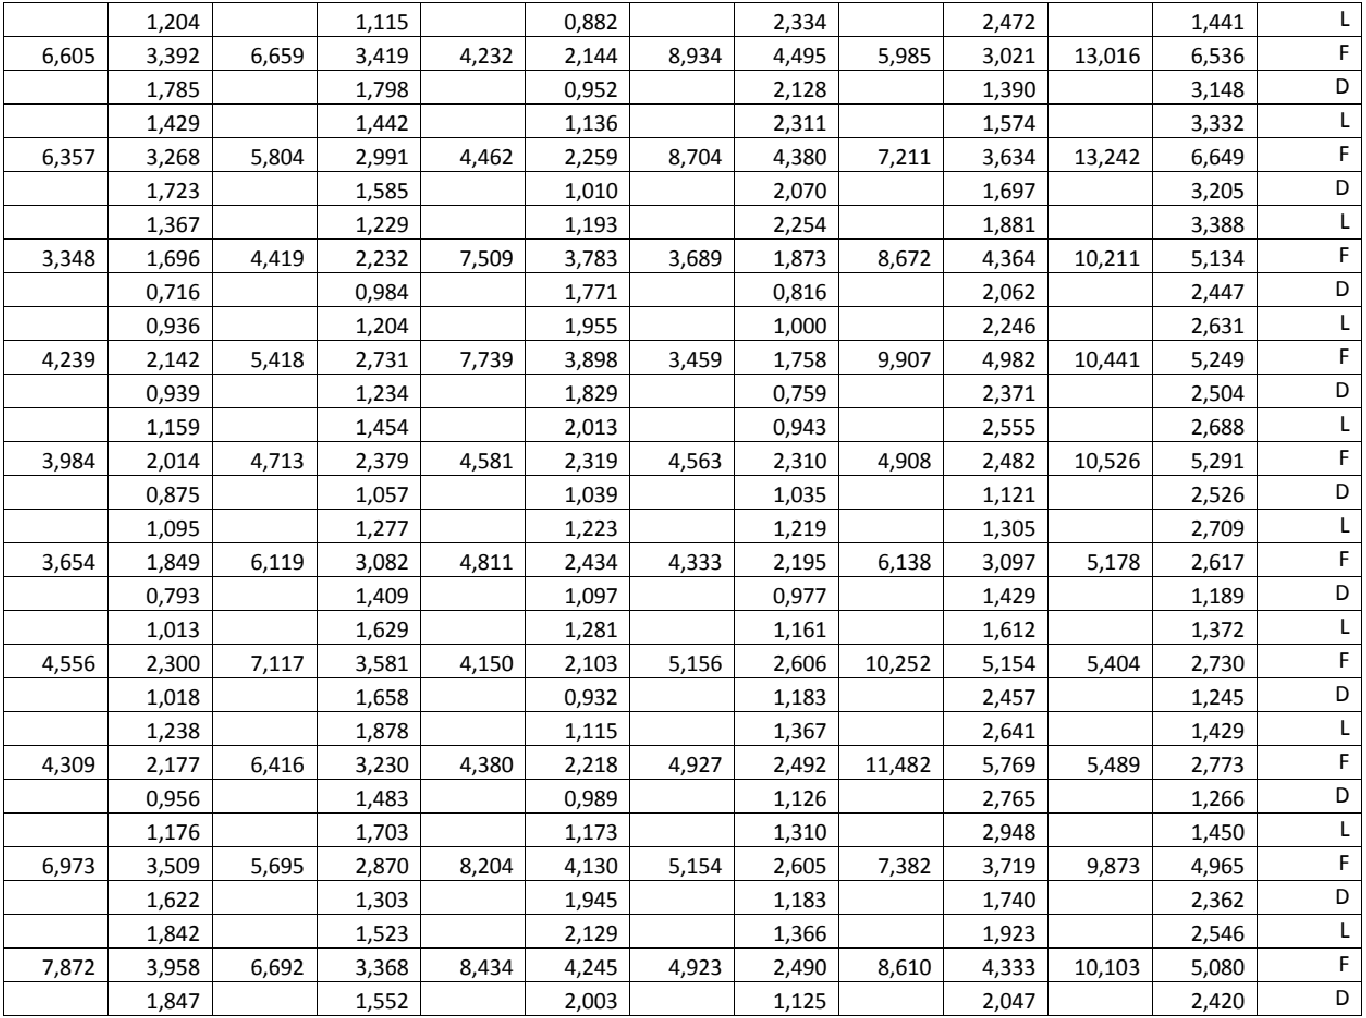
\includegraphics[width=\linewidth]{img/task_2_1}
            \captionof{figure}{Входные данные задачи 2(2)}
        \end{minipage}
    \end{center}
    \begin{center}
        \begin{minipage}{0.9\linewidth}
            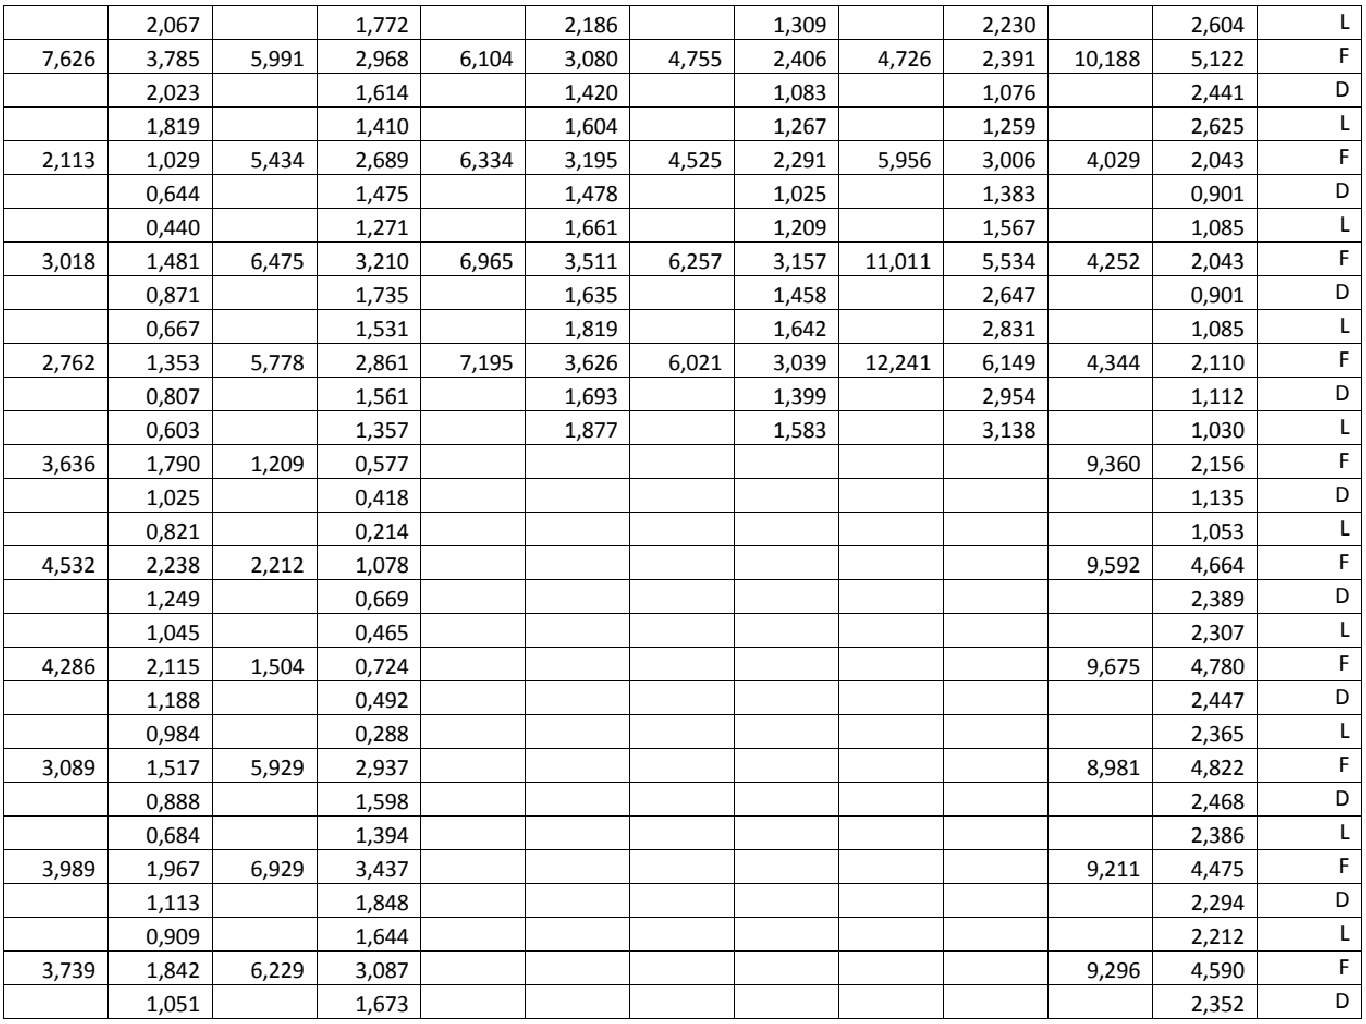
\includegraphics[width=\linewidth]{img/task_2_2}
            \captionof{figure}{Входные данные задачи 2(3)}
        \end{minipage}
    \end{center}
    \begin{center}
        \begin{minipage}{0.9\linewidth}
            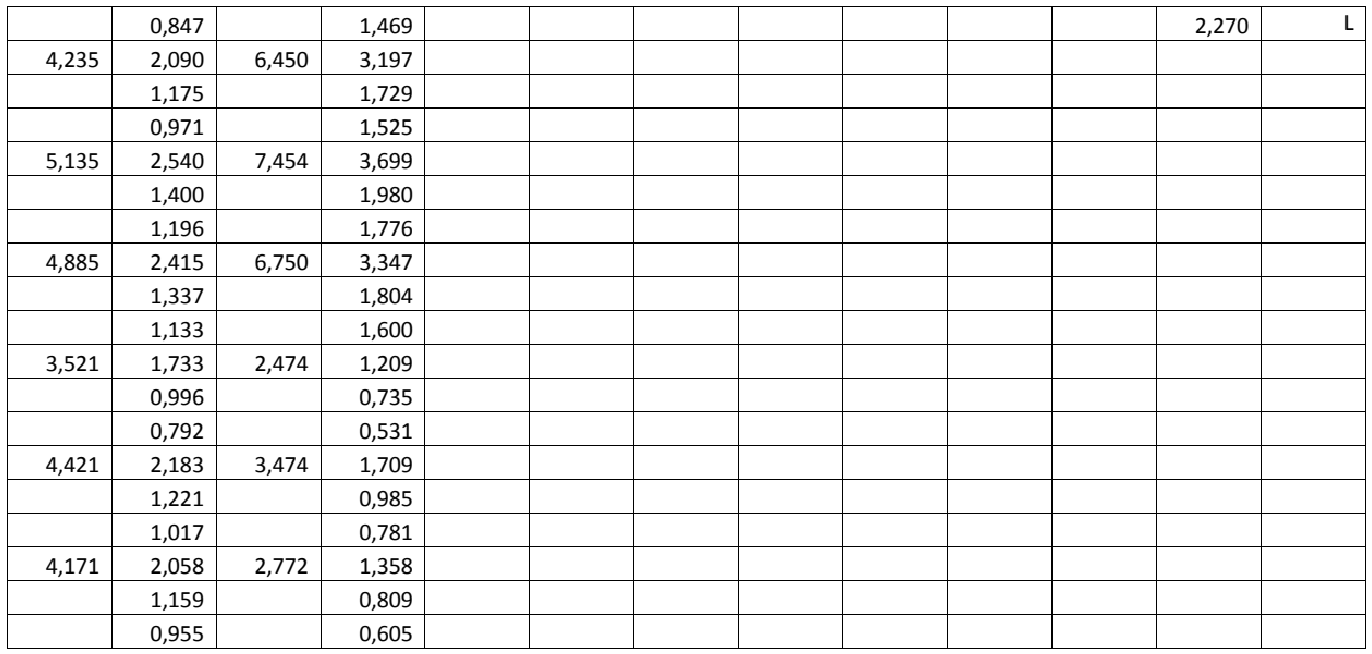
\includegraphics[width=\linewidth]{img/task_2_3}
            \captionof{figure}{Входные данные задачи 2(4)}
        \end{minipage}
    \end{center}


\subsection{Задача 3}
    Найти среднюю стоимость билета пражского метро. Входные данные взять из таблиц, изображенных на рисунках 2-5.
\newpage

\section{Теоретические сведения}
    \textit{\textbf{\underline{Методика построения стохастической модели:}}}
    \begin{enumerate}
        \item Выполняется описание предметной области на естественном языке в общей форме с входными и выходными данными и параметрами системы.
        \item Рисуется схема сложной системы с входными и выходными данными.
        \item Формирование статистической гипотезы относительно распределений потоков входных и выходных данных. Проверка выдвинутых гипотез.
        \item Оценивается возможность реализации модели. При избыточности данных модель упрощается. При недостатке данных изыскивается возможность их получения.
        \item Формируется общее уравнение, связывающее входные и выходные данные.
        \item По результатам эксперимента оцениваются параметры уравнения, полученного на этапе 5.
        \item Оценивается применимость полученной модели на основе контрольных выборок натурного эксперимента для возможности повышения адекватности построенной модели.
        \item Построение концептуальной модели на основе формального описания для проведения натурного эксперимента.
    \end{enumerate}
    
    \textit{\textbf{\underline{Критерий Колмогорова-Смирнова:}}}
    
    Критерий используется для проверки гипотезы $H_0$: "случайная величина $X$ имеет распределение $F(x)$".
    
    Пусть $X_n$ - выборка независимых одинаково распределённых случайных величин, $F_n(x)$ - эмпирическая функция распределения, $F(x)$ - некоторая "истинная" функция распределения с известными параметрами. Статистика критерия определяется выражением:
    \begin{equation}
        D_n=\sup_x |F_n(x)-F(x)|.
    \end{equation}
    
    \textit{\textbf{\underline{Схема пражского метро:}}}
    
    \begin{center}
        \begin{minipage}{0.9\linewidth}
            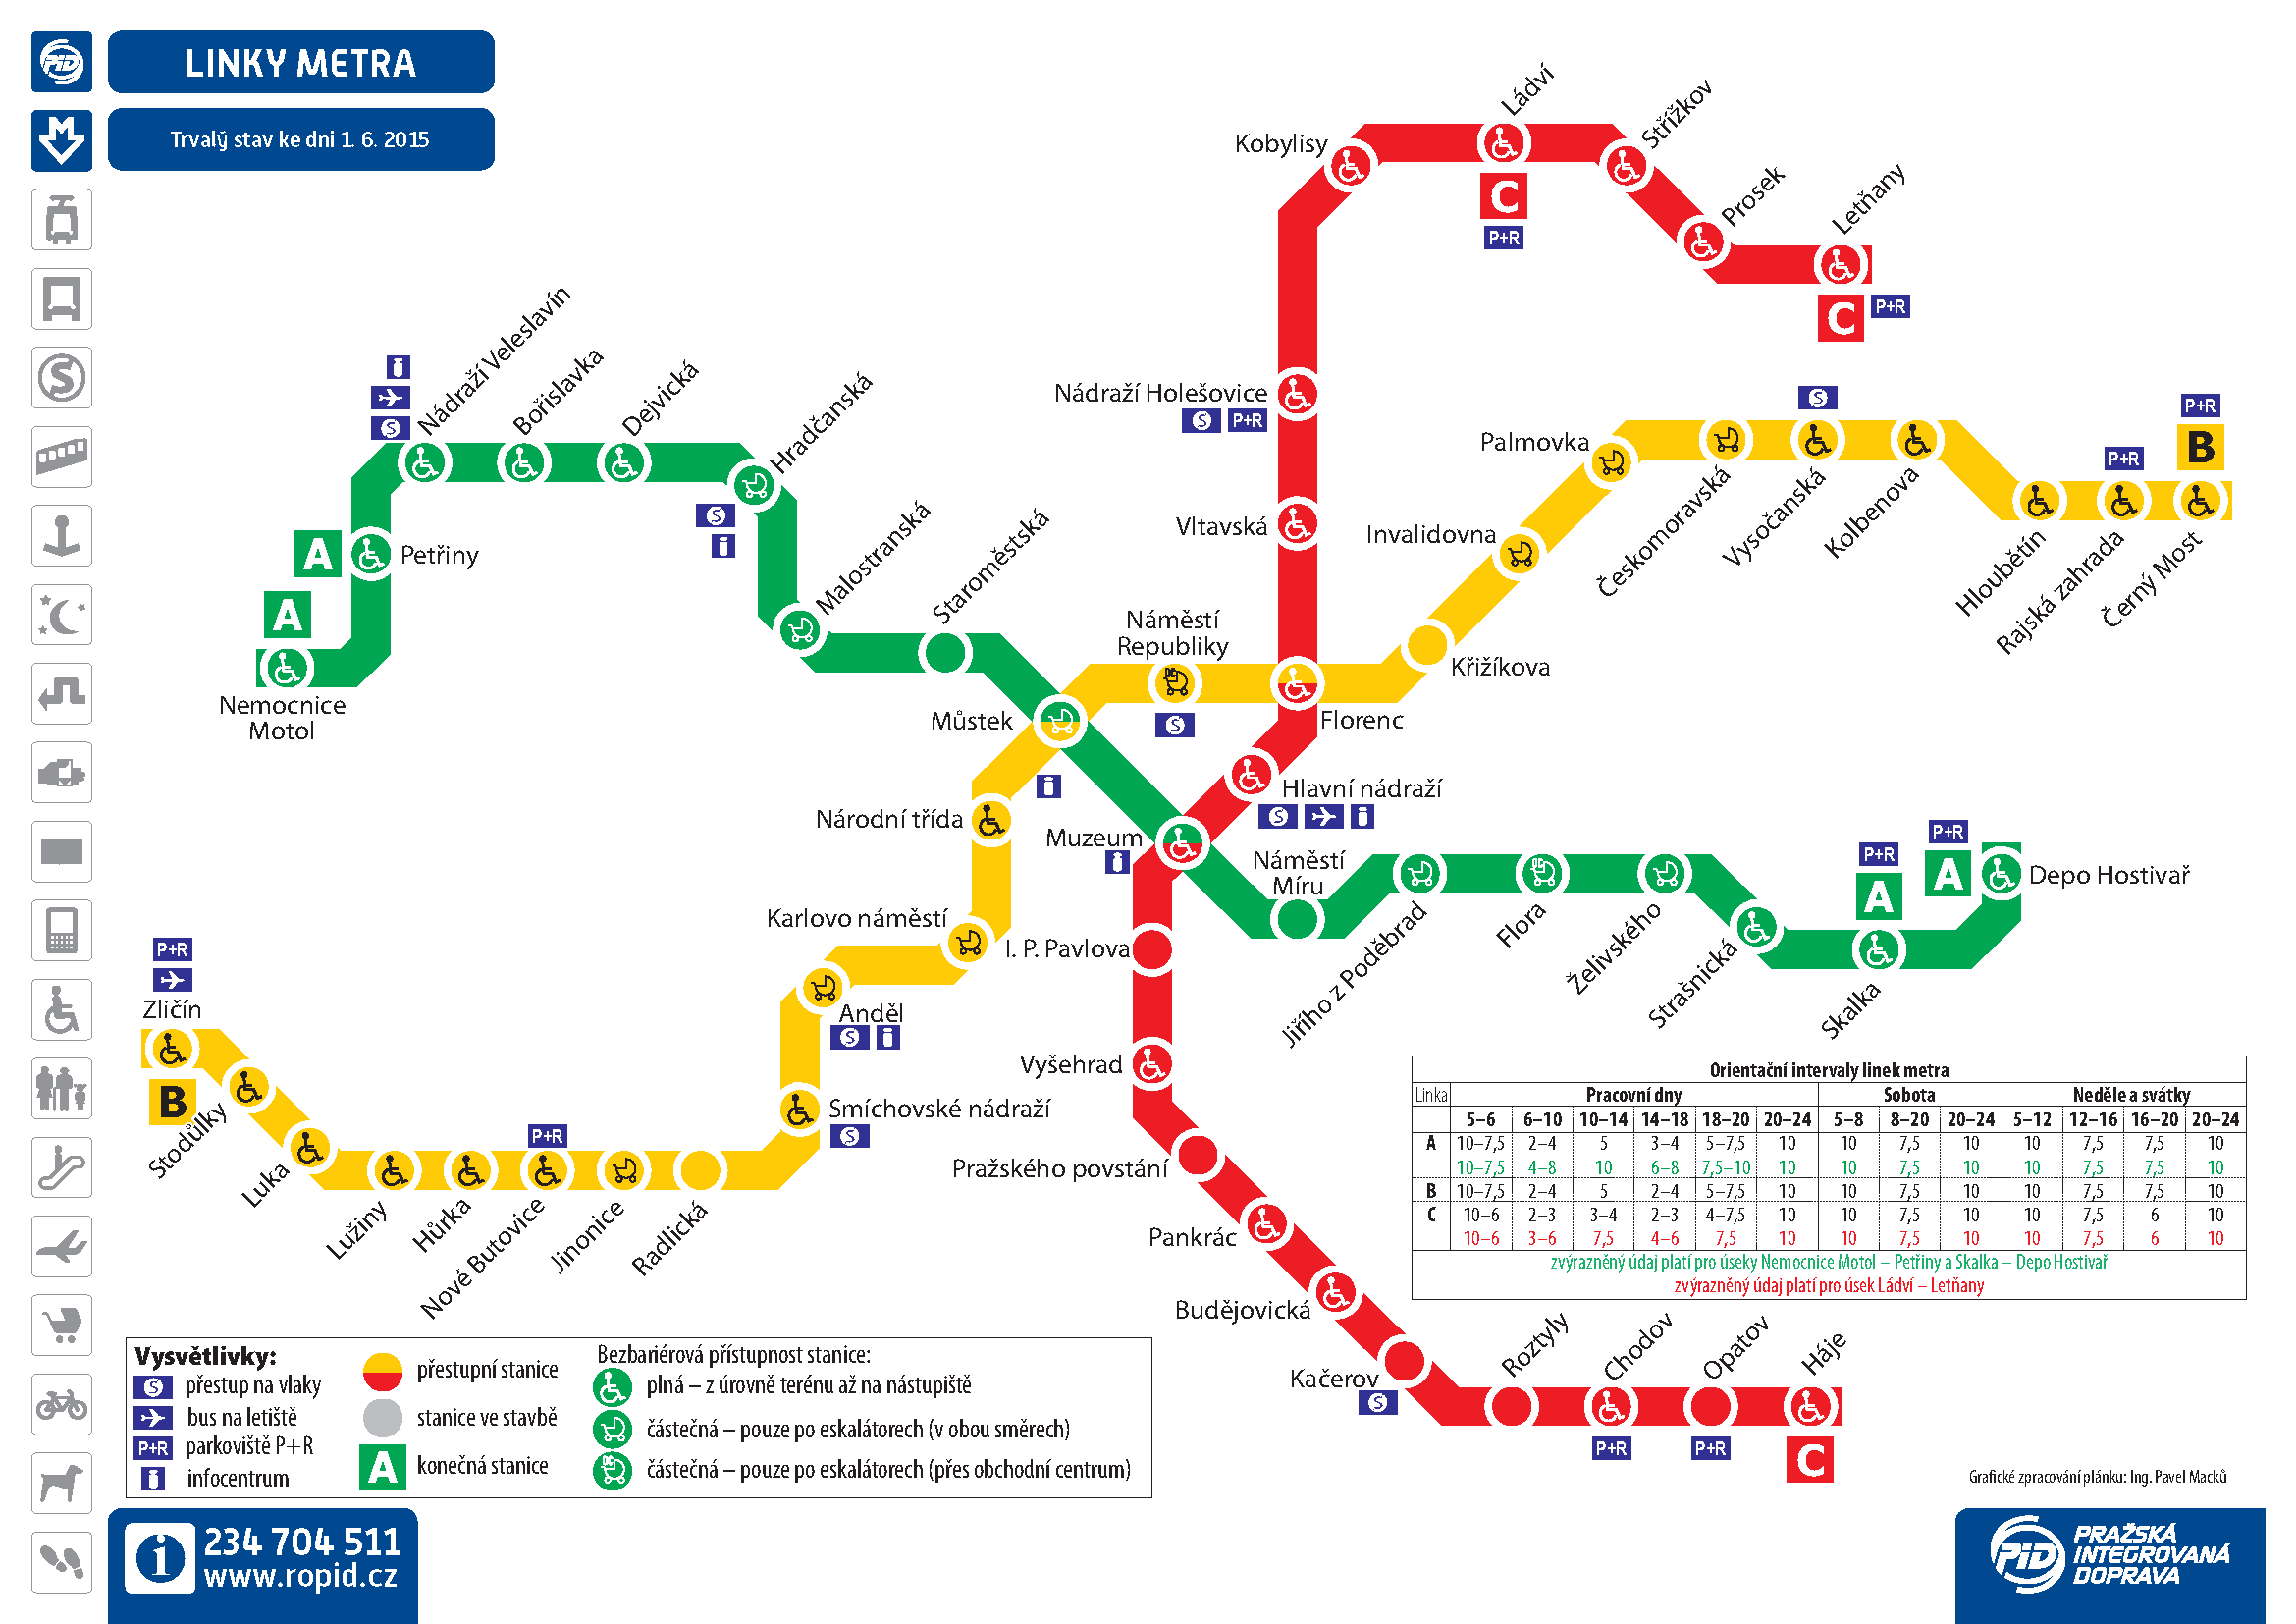
\includegraphics[width=\linewidth]{img/metro-praha}
            \captionof{figure}{Схема метро.}
        \end{minipage}
    \end{center}

    
\subsection{Задача 1}
    Пусть 
    \begin{itemize}
        \item $\varepsilon_1$ - количество людей, вошедших на станцию $Х$ в течение дня;
        \item $\varepsilon_2$ - количество людей, прошедших через турникеты на станции $Х$ в течение дня.
    \end{itemize}
    
    \textit{\textbf{\underline{Гипотеза 1:}}} Между величинами $\varepsilon_1$ и $\varepsilon_2$ существует стохастическая связь, которая может быть выражена как:
    \begin{equation}
        \varepsilon_1 = \varphi(\varepsilon_2) = \alpha \varepsilon_2^\beta.
    \end{equation}
    
    Функция распределения будет иметь вид:
    \begin{equation}
        F(\varepsilon_1, \alpha_1, \beta_1) = 1 - e^{-\lambda_1 \varepsilon_1^{\beta_1}},
    \end{equation}
    \begin{equation}
        F(\varepsilon_2, \alpha_2, \beta_2) = 1 - e^{-\lambda_2 \varepsilon_2^{\beta_2}},
    \end{equation}
    
    Из метода моментов, логарифмируя левую и правую часть равенства, и используя выборочное среднее и среднеквадратичное отклонение для выборок значений случайных величин $\varepsilon_1$ и $\varepsilon_2$, получаем решение для параметров статистик:
    % \begin{equation}
    %     \hat{S}^2(ln (\varepsilon_1)) = \beta^2 \hat{S}^2 (ln(\varepsilon_2))
    % \end{equation}
    \begin{equation}
        \hat{\beta} = \sqrt{\frac{ \hat{S}^2(ln (\varepsilon_1))}{\hat{S}^2 (ln(\varepsilon_2))}}
    \end{equation}
    \begin{equation}
        \hat{\alpha} = exp (\overline{ln (\varepsilon_1)} - \hat{\beta} \overline{ln (\varepsilon_2)}),
    \end{equation}
    где 
    \begin{itemize}
        \item $\hat{\alpha}$ и $\hat{\beta}$ - выборочные значения $\alpha$ и $\beta$,
        \item $ln (\varepsilon_i)$ - средневыборочное значение случайной величины,
        \item $\hat{S}^2$ - среднеквадратичное отклонение выборки.
    \end{itemize}
    
    Далее с помощью критерия Колмогорова-Смирнова можно проверить гипотезу о принадлежности выборки закону распределения 

\subsection{Задача 2}
    Пусть 
    \begin{itemize}
        \item $\varepsilon_1$ - количество людей, вошедших в метро в день контроля;
        \item $\varepsilon_3$ - количество людей, оплативших проезд.
    \end{itemize}
    
    \textit{\textbf{\underline{Гипотеза 2:}}} Существует стохастическая зависимость между случайными величинами $\varepsilon_1$ и $\varepsilon_3$, которую в пределе можно описать функцией вида: 
    \begin{equation}
        \varepsilon_3 = \varphi_2(\varepsilon_2) = \alpha_2 \varepsilon_3^{\beta_2}
    \end{equation}

\subsection{Задача 3}
    Находится количество билетов для каждой категории из трех данных:
    \begin{itemize}
        \item $F$ - взрослый билет ($count\_tickets\_F$);
        \item $D$ - детский билет ($count\_tickets\_D$);
        \item $L$ - льготный билет ($count\_tickets\_L$).
    \end{itemize}
    
    Далее находится среднее арифметическое стоимости билета и общая стоимость всех билетов с помощью формулы:
    \begin{equation}
        cost\_all\_tickets = \sum^{3}_{i=1}{(avg_i * count\_tickets_i)},
    \end{equation}
    где $i = 1$ для $F$, $i = 2$ для $D$, $i = 3$ для $L$.
    
    Тогда средняя стоимость всех билетов будет вычисляться по формуле:
    \begin{equation}
        average = \frac{cost\_all\_tickets}{3 \times \sum^{3}_{i=1}{(count\_tickets_i)}}.
    \end{equation}
    
    



\newpage

\section{Практическая реализация}

\textbf{Листинг 1. Задача 1} 
\begin{minted}[frame=single, framesep=10pt, fontsize = \footnotesize, linenos=true, breaklines]{python}
# work
psi_1w = thA0 + thB0 + thC0
psi_2w = rA0 + rB0 + rC0
alpha, betta = alpha_betta(psi_1w, psi_2w)

print("psi_1: a =", alpha, "b =", betta)

# control
psi_1c = thA1 + thB1 + thC1
psi_2c = rA1 + rB1 + rC1

# _ = *
psi_2_ = psi_2c
psi_1_ = [alpha * (psi_2_[i] ** betta) for i in range(len(psi_2_))]

psi_1c.sort()
psi_1_.sort()

print(get_sections(psi_1c))
print(get_sections(psi_1_))

psi_1c_len = [len(data) / 36 for data in get_sections(psi_1c)]
psi_1__len = [len(data) / 36 for data in get_sections(psi_1_)]

result = [abs(psi_1c_len[i] - psi_1__len[i]) for i in range(len(psi_1c_len))]

if max(result) < 0.05:
	print("Ok")
	print(max(result))
print()
\end{minted}

\textbf{Листинг 2. Задача 2} 
\begin{minted}[frame=single, framesep=10pt, fontsize = \footnotesize, linenos=true, breaklines]{python}
I0 = IIA0 + IIB0 + IIC0

# work
ksi_w1 = []
for value_list in I0:
	ksi_w1.append(sum(map(int, value_list)))

ksi_w2 = []
for value_list in I0:
	if len(value_list) == 3:
		ksi_w2.append(value_list[0] + value_list[1])
	else:
		ksi_w2.append(value_list[0])

ksi_w3 = []
for value_list in I0:
	ksi_w3.append(value_list[len(value_list) - 1])

# control
ksi_c1 = []
for value_list in I0:
	ksi_c1.append(sum(map(int, value_list)))

ksi_c2 = []
for value_list in I0:
	if len(value_list) == 3:
		ksi_c2.append(value_list[0] + value_list[1])
	else:
		ksi_c2.append(value_list[0])

I1 = IIA1 + IIB1 + IIC1

ksi_c3 = []
for value_list in IIA1:
	ksi_c3.append(value_list[len(value_list) - 1])

a_12, b_12 = alpha_betta(ksi_w1, ksi_w2)
a_23, b_23 = alpha_betta(ksi_w2, ksi_w3)

a, b = alpha_betta(ksi_w1, ksi_w3)
print("a_12 = {}, b_12 = {}".format(a_12, b_12))
print("a_23 = {}, b_23 = {}".format(a_23, b_23))

ksi_calc3 = [(x ** (1 / b_23)) / a_23 for x in ksi_c2]
ksi_temp = [a_23 * (x ** b_23) for x in ksi_calc3]
ksi_calc1 = [a_12 * (x ** b_12) for x in ksi_temp]

ksi_c1.sort()
ksi_calc1.sort()
dif = []
n = len(ksi_w1)

for i in range(0, 30, 10):
	func_control = len([x for x in ksi_c1 if x < i]) / n
	func_calc = len([x for x in ksi_calc1 if x < i]) / n
	dif.append(abs(func_control - func_calc))
print("dif ", max(dif))
print()
\end{minted}

\textbf{Листинг 3. Задача 3} 
\begin{minted}[frame=single, framesep=10pt, fontsize = \footnotesize, linenos=true, breaklines]{python}
# work
FDL0 = np.asarray(FDLA0 + FDLB0 + FDLC0)
# FDL1 = FDLA1 + FDLB1 + FDLC1

# F - взрослый
# D - десткий
# L - льготный

count_tickets_F = sum(FDL0[:, 0])
count_tickets_D = sum(FDL0[:, 1])
count_tickets_L = sum(FDL0[:, 2])

avg_F = average(F_30, F_90, F_24, F_72)
avg_D = avg_L = average(D_30, D_90, D_24, D_72)

cost_all_tickets = avg_F * count_tickets_F + avg_D * count_tickets_D + avg_L * count_tickets_L
average_cost = cost_all_tickets / (count_tickets_F + count_tickets_D + count_tickets_L)
print("Average - {}".format(average_cost / 3))
\end{minted}


\newpage
\section{Результаты}
    Ниже приведен результат работы программы из \textbf{Листинга 1, 2, 3}.
    
    \noindent\textbf{Листинг 4.} Результат работы программы для 3 задач.
\begin{minted}[frame=single, framesep=6pt, fontsize = \footnotesize, linenos=true, breaklines]{text}
    --1--
psi_1: a = 1.0644531215676833 b = 1.015231400769257
Hypothesis 1: Ok
0.02777777777777779

	--2--
a_12 = 1.7310412290615682, b_12 = 0.9976777068524383
a_23 = 1.3961675695768274, b_23 = 0.8984112750936865
Hypothesis 2: Ne Ok
0.05555555555555547

	--3--
Average - 19.965618399165084
\end{minted}
    
   \textbf{Задача 1.}
   Гипотеза о наличии связи между между потоком пассажиров, вошедших в метро, и пассажиров, прошедших через турникет подтвердилась, так как критерий Колмогорова-Смирнова дал результат $D = 0.02778$, что соответствует $D < 0.05$ (если $D > 0.05$ - то гипотеза бы не подтвердилась). 
   
   \textbf{Задача 2.}
   Гипотеза о наличии связи между между кол-вом людей, вошедших в метро в день контроля, и кол-вом людей, оплатвших проезд не подтвердилась, так как критерий Колмогорова-Смирнова дал результат $D = 0.0556$ ($D > 0.05$).
   
   \textbf{Задача 3.}
   Была получена средняя стоимость билета пражского метро - $19.97$ крон.


\newpage
\section{Вывод}
    В ходе лабораторной работы была изучена стохастическая модель на примере пражского метро, применен критерий Колмогорова-Смирнова, получена средняя стоимость билета метро на основе входных данных, полученных с помощью натурного эксперимента. 


\end{document} 














